%%%%%%%%%%%%%%%%%%%%%%%%%%%%%%%%%%%%%%%%%%%%%%%%%%%%%%%%%%%%%%%%%%%%%%%%

\begin{slide}{}
\normalsize

\begin{center}
Analyse der naiven Methode
\end{center}
\vspace*{0.5cm}

\footnotesize
\begin{enumerate}
\item Sei $n$ Zahl der Eintr\"age im Telefon--Buch.
\item Aufwand, um neuen Eintrag hinzuzuf\"ugen: \\[0.3cm]
      \hspace*{1.3cm} $\Oh(1)$
\item Aufwand, um Eintrag nachzuschlagen: \\[0.3cm]
      \hspace*{1.3cm} $\Oh(1)$
\item Aufwand, um Telefon--Buch aufzubauen:  \\[0.3cm]
      \hspace*{1.3cm} $\Oh(n)$
\end{enumerate}
\vspace*{0.3cm}

\begin{center}
   \framebox{ \framebox{Besser gehts nicht!} }
\end{center}

\vspace*{0.3cm}
Probleme der naiven Methode:
\begin{enumerate}
\item Braucht sehr, sehr viel Speicher!
\item Funktioniert nicht, wenn Namen mehr als 10 \\
      Buchstaben haben.
\item In der Funktion \texttt{computeIndex} tritt Überlauf ein.
\end{enumerate}


\vspace*{\fill}
\tiny \addtocounter{mypage}{1}
\rule{17cm}{1mm}
Hashing  \hspace*{\fill} Seite \arabic{mypage}
\end{slide}

%%%%%%%%%%%%%%%%%%%%%%%%%%%%%%%%%%%%%%%%%%%%%%%%%%%%%%%%%%%%%%%%%%%%%%%%

\begin{slide}{}
\normalsize

\begin{center}
Hashing
\end{center}
\vspace*{0.5cm}

\footnotesize
Ziel: Entwicklung einer Methode, die 
\begin{enumerate}
\item im statistischen Mittel vergleichbare Performanz hat wie die naive Methode
\item Speicherverbrauch: $\Oh(n)$
\end{enumerate}

Erster Versuch:
\begin{enumerate}
\item Anlegen eines Feldes der Gr\"o{\ss}e $n$ \\[0.3cm]
      \hspace*{1.3cm} $\texttt{unsigned telephone[}n\mathtt{];}$
\item Berechnung des Index
\begin{verbatim} 
unsigned computeIndex(const char text[], unsigned n) 
{
    unsigned index = 0;
    for (unsigned i = 0; i < 10; ++i) {
        index = (128 * index + text[i]) % n;
    }
    return index;
}
\end{verbatim}
\item Speichere Telefon--Nummer unter berechneten Index: \\[0.3cm]
      \hspace*{1.3cm} $\texttt{index = computeIndex(name,} n\mathtt{);}$ \\[0.3cm]
      \hspace*{1.3cm} \texttt{telephone[index] = telNumber;}
\item Suchen: Berechne Index des gegebenen Namens: \\[0.3cm]
      \hspace*{1.3cm} $\texttt{index = computeIndex(name,} n\mathtt{);}$ \\[0.3cm]
      \hspace*{1.3cm} $\texttt{telNumber = telephone[index]}$
\end{enumerate}

\vspace*{\fill}
\tiny \addtocounter{mypage}{1}
\rule{17cm}{1mm}
Hashing  \hspace*{\fill} Seite \arabic{mypage}
\end{slide}

%%%%%%%%%%%%%%%%%%%%%%%%%%%%%%%%%%%%%%%%%%%%%%%%%%%%%%%%%%%%%%%%%%%%%%%%

\begin{slide}{}
\normalsize

\begin{center}
Analyse des 1. Versuchs
\end{center}
\vspace*{0.5cm}

\footnotesize
\begin{enumerate}
\item Performanz: \textbf{ok}
\item Speicher--Verbrauch: Feld der L\"ange $n$: \textbf{ok}
\item \textbf{Korrektheit}? \textbf{Nein}!
\end{enumerate}

\textbf{Problem}: Kollisionen
\begin{verbatim}
    computeIndex( "Pfennig",   22 ) = 12
    computeIndex( "Schlensog", 22 ) = 12
\end{verbatim}
Verschiedene Sch\"ussel k\"onnen auf den gleichen Wert 
abgebildet werden!
\vspace*{0.5cm}

\textbf{L\"osung}: Feld \texttt{telephone} enth\"alt nicht 
\begin{itemize}
\item Telefon--Nummer, sondern
\item Zeiger auf verkette Liste mit Paaren $\langle \mathtt{Name}, \mathtt{telNr} \rangle$
\item Diese Listen dienen als Dictionary!
\end{itemize}
Suchen nun in zwei Stufen:
\begin{enumerate}
\item Berechnung des Index \\[0.3cm]
     \hspace*{1.3cm} \texttt{computeIndex(key, n);}
\item Suche in verketteter Liste \texttt{telephone[index]} \\[0.3cm]
     \hspace*{1.3cm} \texttt{search(telephone[index], key)}
\end{enumerate}
Einf\"ugen und L\"oschen analog

\vspace*{\fill}
\tiny \addtocounter{mypage}{1}
\rule{17cm}{1mm}
Hashing  \hspace*{\fill} Seite \arabic{mypage}
\end{slide}

%%%%%%%%%%%%%%%%%%%%%%%%%%%%%%%%%%%%%%%%%%%%%%%%%%%%%%%%%%%%%%%%%%%%%%%%

\begin{slide}{}
\normalsize

\begin{center}
Hash--Tabelle mit getrennter Verkettung
\end{center}
\vspace*{0.5cm}

\footnotesize
\epsfig{file=hash-table.ps}


\vspace*{\fill}
\tiny \addtocounter{mypage}{1}
\rule{17cm}{1mm}
Hashing  \hspace*{\fill} Seite \arabic{mypage}
\end{slide}

%%%%%%%%%%%%%%%%%%%%%%%%%%%%%%%%%%%%%%%%%%%%%%%%%%%%%%%%%%%%%%%%%%%%%%%%

\begin{slide}{}
\normalsize

\begin{center}
Implementierung in C
\end{center}
\vspace*{0.5cm}

\footnotesize
Hash--Tabelle ben\"otigt folgende Daten
\begin{enumerate}
\item Zahl der Eintr\"age \\[0.3cm]
      \hspace*{1.3cm} \texttt{unsigned noEntries;}
\item Gr\"o{\ss}e des angelegten Feldes \\[0.3cm]
      \hspace*{1.3cm} \texttt{unsigned noBuckets;}
\item Feld mit Zeigern auf Listen--Knoten \\[0.3cm]
      \hspace*{1.3cm} \texttt{List* table;}
\end{enumerate}
Also Definition der Daten--Struktur wie folgt:
\begin{verbatim}
    typedef struct {
        unsigned noEntries; 
        unsigned noBuckets; 
        List*    table;     
    } HashTable;
\end{verbatim}
\vspace*{0.3cm}

\textbf{Definition}: \emph{Auslastungs--Faktor} (load factor) \\[0.3cm]
\hspace*{1.3cm} $\alpha = \bruch{\mathtt{noEntries}}{\mathtt{noBuckets}}$
\vspace*{0.5cm}

Falls Hash--Funktion die Schl\"ussel gut \"uber Tabelle verteilt, gibt $\alpha$
mittlere L\"ange der Listen an.

Praxis: $\alpha \leq 4$ ist gute Wahl.

\vspace*{\fill}
\tiny \addtocounter{mypage}{1}
\rule{17cm}{1mm}
Hashing  \hspace*{\fill} Seite \arabic{mypage}
\end{slide}

%%%%%%%%%%%%%%%%%%%%%%%%%%%%%%%%%%%%%%%%%%%%%%%%%%%%%%%%%%%%%%%%%%%%%%%%

\begin{slide}{}
\normalsize

\begin{center}
Implementierung (Fortsetzung)
\end{center}
\vspace*{0.5cm}

\footnotesize
\begin{enumerate}
\item Suchen
      \begin{verbatim}
Value* searchTable(HashTable* htPtr, Key key) 
{
    unsigned index = hash(key, htPtr->noBuckets);
    return search(htPtr->table[index], key);
}
      \end{verbatim}
\item Einf\"ugen
\begin{verbatim}
void insertTable(HashTable* htPtr, Key key, Value val)
{
    ++(htPtr->noEntries);
    unsigned index = hash(key, htPtr->noBuckets);
    htPtr->table[index] = 
        insert(htPtr->table[index], key, val);
}
\end{verbatim}
\item L\"oschen
\begin{verbatim}
void deleteTable(HashTable* htPtr, Key key) 
{
    --(htPtr->noEntries);
    unsigned index = hash(key, htPtr->noBuckets);
    htPtr->table[index] = 
        delete(htPtr->table[index], key);
}
\end{verbatim}
\end{enumerate}

\vspace*{\fill}
\tiny \addtocounter{mypage}{1}
\rule{17cm}{1mm}
Hashing  \hspace*{\fill} Seite \arabic{mypage}
\end{slide}

%%%%%%%%%%%%%%%%%%%%%%%%%%%%%%%%%%%%%%%%%%%%%%%%%%%%%%%%%%%%%%%%%%%%%%%%

\begin{slide}{}
\normalsize

\begin{center}
Anlegen der Hash--Tabelle
\end{center}
\vspace*{0.5cm}

\footnotesize
Anlegen einer Hash--Tabelle mit \texttt{size} Buckets
\begin{verbatim}
HashTable* makeTable(unsigned size) {
    HashTable* ht = malloc( sizeof(HashTable) );
    unsigned index = 0;
    unsigned count = primes[index];
    while (count < size) {
        count = primes[++index];
    }
    ht->noBuckets = count;
    ht->noEntries = 0;
    ht->table = malloc( sizeof(NodePtr) * count );
    for (unsigned i = 0; i < ht->noBuckets; ++i) {
        ht->table[i] = 0;
    }
    return ht;
}
\end{verbatim}
\begin{enumerate}
\item \texttt{primes}: Feld, was wachsende Primzahlen enth\"alt.

      $\mathtt{primes}[i+1] \approx 2 * \mathtt{primes}[i]$
\item \texttt{index} wird hochgez\"ahlt, bis Primzahl \texttt{count} gefunden ist,
      die Gr\"o{\ss}er als \texttt{size} ist.
\item Dann wird Feld der Gr\"o{\ss}e \texttt{count} angelegt.
\item Feld wird mit 0--Pointern initialisiert.

      (0--Pointer $\widehat{=}$ leere Liste)
\end{enumerate}


\vspace*{\fill}
\tiny \addtocounter{mypage}{1}
\rule{17cm}{1mm}
Hashing  \hspace*{\fill} Seite \arabic{mypage}
\end{slide}

%%%%%%%%%%%%%%%%%%%%%%%%%%%%%%%%%%%%%%%%%%%%%%%%%%%%%%%%%%%%%%%%%%%%%%%%

\begin{slide}{}
\normalsize

\begin{center}
Komplexit\"at 
\end{center}
\vspace*{0.5cm}

\footnotesize
Absch\"atzung der Komplexit\"aten f\"ur naives \emph{Hashing}

$n$: Zahl der Eintr\"age in Hash--Tabelle

$\alpha$: Auslastungs--Faktor
\begin{enumerate}
\item Suche:    
  \begin{enumerate}
  \item Worst Case                 \hspace*{6.0cm} $n \in \Oh(n)$
  \item Statistischer Durchschnitt \hspace*{1.3cm} $\bruch{\alpha}{2} \in \Oh(1)$ 
  \end{enumerate}
\item L\"oschen: 
  \begin{enumerate}
  \item Worst Case                 \hspace*{6.0cm} $n \in \Oh(n)$
  \item Statistischer Durchschnitt \hspace*{1.3cm} $\bruch{\alpha}{2} \in \Oh(1)$ 
  \end{enumerate}
\item Einf\"ugen: \hspace*{1.3cm}   
  \begin{enumerate}
  \item Worst Case                 \hspace*{7.2cm} $\Oh(1)$
  \item Statistischer Durchschnitt \hspace*{2.9cm} $\Oh(1)$ 
  \end{enumerate}
\end{enumerate}
\textbf{Worst Case}: 
\begin{enumerate}
\item Hash--Funktion berechnet immer selben Index
\item Alle $n$ Eintr\"age in einer Zeile
\end{enumerate}
\textbf{Statistischer Mittelwert}
\begin{enumerate}
\item Jede Zeile enth\"alt im Durchschnitt $\alpha$ Eintr\"age
\end{enumerate}

\vspace*{\fill}
\tiny \addtocounter{mypage}{1}
\rule{17cm}{1mm}
Hashing  \hspace*{\fill} Seite \arabic{mypage}
\end{slide}

%%%%%%%%%%%%%%%%%%%%%%%%%%%%%%%%%%%%%%%%%%%%%%%%%%%%%%%%%%%%%%%%%%%%%%

\begin{slide}{}
\normalsize

\begin{center}
Hash--Funktion
\end{center}
\vspace*{0.5cm}

\footnotesize

\textbf{Definition}: \\[0.3cm]
\emph{Hash--Funktion} berechnet zu gegeb. Schl\"ussel den Index: \\[0.3cm]
\hspace*{1.3cm} $\textsl{hash}: \textsl{Key} \rightarrow \mathbb{N}$

\textbf{Anforderungen}:
\begin{enumerate}
\item Ist $n$ Gr\"o{\ss}e der Tabelle, so muss gelten: \\[0.3cm]
      \hspace*{1.3cm} $\textsl{hash}(k) < n$
\item Schl\"ussel sollen m\"oglichst gleichm\"a{\ss}ig auf Tabelle verteilt werden
\item Hash--Funktion soll einfach zu berechnen sein
\end{enumerate}
Gebr\"auchliche Hash--Funktionen
\begin{enumerate}
\item Divisions--Methode \\[0.3cm]
      \hspace*{1.3cm} $\textsl{hash}(k) \;=\; k\;\%\; n$ \\[0.3cm]
      Dabei sollte Tabellen--Gr\"o{\ss}e $n$  Primzahl sein!
\item Multiplikations--Methode: Sei $k\in\mathbb{R}$ \\[0.3cm]
      \hspace*{1.3cm} $\mathtt{floor}\bigg(n * \mathtt{fract}(A * k) \bigg)$ 
      \begin{enumerate}
      \item $\mathtt{floor}(x)$: gr\"o{\ss}te nat\"urliche Zahl kleiner $x$
      \item $\mathtt{fract}(x) := x - \mathtt{floor}(x)$
      \item $A := \bruch{\sqrt{5} - 1}{2} \approx 0.61803398875$    
      \end{enumerate}
\end{enumerate}


\vspace*{\fill}
\tiny \addtocounter{mypage}{1}
\rule{17cm}{1mm}
Hashing  \hspace*{\fill} Seite \arabic{mypage}
\end{slide}

%%%%%%%%%%%%%%%%%%%%%%%%%%%%%%%%%%%%%%%%%%%%%%%%%%%%%%%%%%%%%%%%%%%%%%%%

\begin{slide}{}
\normalsize

\begin{center}
Hash--Funktion f\"ur Strings
\end{center}
\vspace*{0.5cm}

\footnotesize

\begin{verbatim}
    int hash(const char* key, unsigned size) {
        const    char* ptr;
        unsigned result;
        result = 0;
        ptr    = key;
        while (*ptr != '\0') {
            result = (result << 4) + (*ptr);
            unsigned tmp = result & 0xf0000000;
            if (tmp != 0) {
                result = result ^ (tmp >> 24);
                result = result ^ tmp;
            }
            ptr++;
        }
        return result % size;
    }
\end{verbatim}
\begin{enumerate}
\item Alle Buchstaben werden ber\"ucksichtigt
\item Verschiedene Bits der Buchstaben werden durch die Operationen 
      \texttt{\^} (exklusives Oder) und Addition vermischt
\item Wird in der Praxis f\"ur Symbol--Tabellen in Compilern
      eingesetzt.

      (siehe auch Aho, Sethi, Ullmann: \\[0.3cm]
      \hspace*{1.3cm} \emph{Compilers: Principles, Techniques, and Tools})
\end{enumerate}

\vspace*{\fill}
\tiny \addtocounter{mypage}{1}
\rule{17cm}{1mm}
Hashing  \hspace*{\fill} Seite \arabic{mypage}
\end{slide}


%%%%%%%%%%%%%%%%%%%%%%%%%%%%%%%%%%%%%%%%%%%%%%%%%%%%%%%%%%%%%%%%%%%%%%%%

\begin{slide}{}
\normalsize

\begin{center}
Kritik der bisherigen Methode
\end{center}
\vspace*{0.5cm}

\footnotesize
Probleme der Implementierung:
\begin{enumerate}
\item Bisher vorgestelltes Verfahren setzt Kenntnis 
      der maximalen Anzahl von Eintr\"agen in Tabelle voraus
\item Wird Tabelle zu klein gew\"ahlt: \\[0.3cm]
      \hspace*{1.3cm} \textbf{schlechte Performanz}
\item Wird Tabelle zu gro{\ss} gew\"ahlt: \\[0.3cm]
      \hspace*{1.3cm} \textbf{Verschwendung von Speicherplatz}
\item Falls Zahl der Eintr\"age mit der Zeit w\"achst, kann
      der Auslastungs--Faktor gar nicht optimal eingestellt werden:
      \begin{enumerate}
      \item entweder ist die Tabelle am Anfang zu gro{\ss}
      \item oder die Tabelle ist sp\"ater zu klein
      \end{enumerate}
\end{enumerate}

\textbf{L\"osung}: Tabelle muss dynamisch wachsen k\"onnen
\begin{enumerate}
\item Bei jedem Einf\"ugen kontrollieren des Auslastungs--Faktors $\alpha$
\item Falls $\alpha > 4$ \emph{Rehashing}: 
  \begin{enumerate}
  \item Lege doppelt so gro{\ss}e neue Tabelle an
  \item Kopiere alte Tabelle in neue Tabelle
  \end{enumerate}
\end{enumerate}


\vspace*{\fill}
\tiny \addtocounter{mypage}{1}
\rule{17cm}{1mm}
Hashing  \hspace*{\fill} Seite \arabic{mypage}
\end{slide}

%%%%%%%%%%%%%%%%%%%%%%%%%%%%%%%%%%%%%%%%%%%%%%%%%%%%%%%%%%%%%%%%%%%%%%%%

\begin{slide}{}
\normalsize

\begin{center}
Implementierung Rehashing
\end{center}
\vspace*{0.5cm}

\footnotesize
\begin{verbatim}
HashTable* rehash(HashTable* htPtr) {
    HashTable* newTable = 
        makeTable(htPtr->noBuckets * 2);
    newTable->noEntries = htPtr->noEntries;
    for (unsigned idx = 0; idx < htPtr->noBuckets; ++idx) 
    {
        NodePtr nodePtr = htPtr->table[idx];
        while (nodePtr != 0) {
            Key      key   = nodePtr->key;
            Value    val   = nodePtr->val;
            unsigned index = 
                hash(key, newTable->noBuckets);
            newTable->table[index] = 
                insert(newTable->table[index], key, val);
            nodePtr = nodePtr->nextPtr;
        }
    }
    freeHashTable(htPtr);
    free(htPtr);
    return newTable;
}
\end{verbatim}
Algorithmus
\begin{enumerate}
\item neue Tabelle anlegen
\item alte Tabelle Zeile f\"ur Zeile durchgehen
\item jeden Eintrag aus alter Tabelle in neue Tabelle einf\"ugen
\item alte Tabelle l\"oschen
\end{enumerate}

\vspace*{\fill}
\tiny \addtocounter{mypage}{1}
\rule{17cm}{1mm}
Hashing  \hspace*{\fill} Seite \arabic{mypage}
\end{slide}

%%%%%%%%%%%%%%%%%%%%%%%%%%%%%%%%%%%%%%%%%%%%%%%%%%%%%%%%%%%%%%%%%%%%%%%%

\begin{slide}{}
\normalsize

\begin{center}
Komplexit\"at 
\end{center}
\vspace*{0.5cm}

\footnotesize
Absch\"atzung der Komplexit\"aten f\"ur \emph{dynamisches Hashing}

Sei $n$ Zahl der Eintr\"age in Hash--Tabelle
\begin{enumerate}
\item Suche:    
  \begin{enumerate}
  \item Worst Case                 \hspace*{7.2cm} $\Oh(n)$
  \item Statistischer Durchschnitt \hspace*{2.9cm} $\Oh(1)$ 
  \end{enumerate}
\item L\"oschen: 
  \begin{enumerate}
  \item Worst Case                 \hspace*{7.2cm} $\Oh(n)$
  \item Statistischer Durchschnitt \hspace*{2.9cm} $\Oh(1)$ 
  \end{enumerate}
\item Einf\"ugen: \hspace*{1.3cm}   
  \begin{enumerate}
  \item Worst Case                 \hspace*{7.2cm} $\Oh(n)$
  \item Statistischer Durchschnitt \hspace*{1.5cm} $\Oh\bigg(\log(n)\bigg)$ 
  \end{enumerate}
\end{enumerate}
\textbf{Worst Case}: 
\begin{enumerate}
\item Hash--Funktion berechnet immer selben Index
\item Alle $n$ Eintr\"age in einer Zeile
\end{enumerate}
\textbf{Statistischer Mittelwert}
\begin{enumerate}
\item Jede Zeile enth\"alt $\alpha$ Eintr\"age
\item $\alpha < 4$
\end{enumerate}

\vspace*{\fill}
\tiny \addtocounter{mypage}{1}
\rule{17cm}{1mm}
Hashing  \hspace*{\fill} Seite \arabic{mypage}
\end{slide}

%%%%%%%%%%%%%%%%%%%%%%%%%%%%%%%%%%%%%%%%%%%%%%%%%%%%%%%%%%%%%%%%%%%%%%%%%

%\begin{slide}{}
%\normalsize

%\begin{center}
%\end{center}
%\vspace*{0.5cm}

%\footnotesize


%\vspace*{\fill}
%\tiny \addtocounter{mypage}{1}
%\rule{17cm}{1mm}
%Hashing  \hspace*{\fill} Seite \arabic{mypage}
%\end{slide}


%%% Local Variables: 
%%% mode: latex
%%% TeX-master: "hashing.tex"
%%% TeX-master: "hashing"
%%% End: 
